\documentclass[12pt]{article}

%-------------PACKAGES------------- 
\usepackage[margin=1in]{geometry} 
\usepackage{amsmath,amsthm,amssymb}
\usepackage{pgfplots}
\usepackage{float}
\usepackage{braket}
\usepackage{titling}
\usepackage{wrapfig}
\usepackage{tikz}
\usepackage{mwe}
\usepackage{enumitem}
\usepackage{mathtools}
\usepackage{scrextend}
\usepackage{listings}
\usepackage{color}
\usepackage{caption}
\usepackage{subcaption}
\usepackage{algorithm,algpseudocode}
\usetikzlibrary{shapes,arrows,chains}
\usetikzlibrary[calc]

%-------------FORMATTING-------------
\setlength{\droptitle}{-7.5em} 
\setlength{\parindent}{0pt}
\def\LW{\dimexpr.25\linewidth-.5em} 
\tikzstyle{line} = [draw, -latex']

%--------------COMMANDS--------------
\newcommand{\N}{\mathbb{N}}
\newcommand{\Z}{\mathbb{Z}}
\newcommand{\R}{\mathbb{R}}
\newcommand{\C}{\mathbb{C}}
%\renewcommand{\qedsymbol}{\filledbox}

\DeclarePairedDelimiter \abs{\lvert}{\rvert}%
\DeclarePairedDelimiter \babs{\bigg\lvert}{\bigg\rvert}%
\DeclarePairedDelimiter \norm{\lVert}{\rVert}%

%------------ENVIRONMENTS------------- 
\newenvironment{theorem}[2][]{\begin{trivlist}
		\item[{\bfseries #1}\hskip \labelsep {\bfseries #2.}]}{\end{trivlist}}
\newenvironment{lemma}[2][Lemma]{\begin{trivlist}
		\item[\hskip \labelsep {\bfseries #1}\hskip \labelsep {\bfseries #2.}]}{\end{trivlist}}
\newenvironment{exercise}[2][Exercise]{\begin{trivlist}
		\item[\hskip \labelsep {\bfseries #1}\hskip \labelsep {\bfseries #2.}]}{\end{trivlist}}
\newenvironment{reflection}[2][Reflection]{\begin{trivlist}
		\item[\hskip \labelsep {\bfseries #1}\hskip \labelsep {\bfseries #2.}]}{\end{trivlist}}
\newenvironment{proposition}[2][Proposition]{\begin{trivlist}
		\item[\hskip \labelsep {\bfseries #1}\hskip \labelsep {\bfseries #2.}]}{\end{trivlist}}
\newenvironment{corollary}[2][Corollary]{\begin{trivlist}
		\item[\hskip \labelsep {\bfseries #1}\hskip \labelsep {\bfseries #2.}]}{\end{trivlist}}
\newenvironment{definition}[2][]{\begin{trivlist}
		\item[{\bfseries #1}\hskip \labelsep {\bfseries #2.}]}{\end{trivlist}}
\theoremstyle{remark}
\newtheorem*{remark}{Remark}

%-------------CODE-STYLE------------
\definecolor{dkgreen}{rgb}{0,0.6,0}
\definecolor{gray}{rgb}{0.5,0.5,0.5}
\definecolor{mauve}{rgb}{0.58,0,0.82}
\lstset{frame=tb,
	language=C++,
	aboveskip=3mm,
	belowskip=3mm,
	showstringspaces=false,
	columns=flexible,
	basicstyle={\small\ttfamily},
	numbers=none,
	numberstyle=\tiny\color{gray},
	keywordstyle=\color{blue},
	commentstyle=\color{dkgreen},
	stringstyle=\color{mauve},
	breaklines=true,
	breakatwhitespace=true,
	tabsize=3
}

\tikzset{
	path image/.style={
		path picture={
			\node at (path picture bounding box.center) {
				\includegraphics[height=3cm]{example-image}};}},
	path tikzimage/.style={
		path picture={
			\node at (path picture bounding box.center)
			[circle, fill=blue!50, scale=2, text=yellow]{Bravo};}}
}

\lstset{
	morekeywords={end}
}

%------------------------------------ 
%---------START-OF-DOCUMENT----------
%------------------------------------
\begin{document}
	
	\title{Paper Summary}
	\author{David Miller \\ 
		CIS 5930: Social Network Mining} 
	
	\maketitle 
	
	\begin{figure}[H]{}
		\centering
		\vspace{-15pt}
		\hspace{-10pt}
		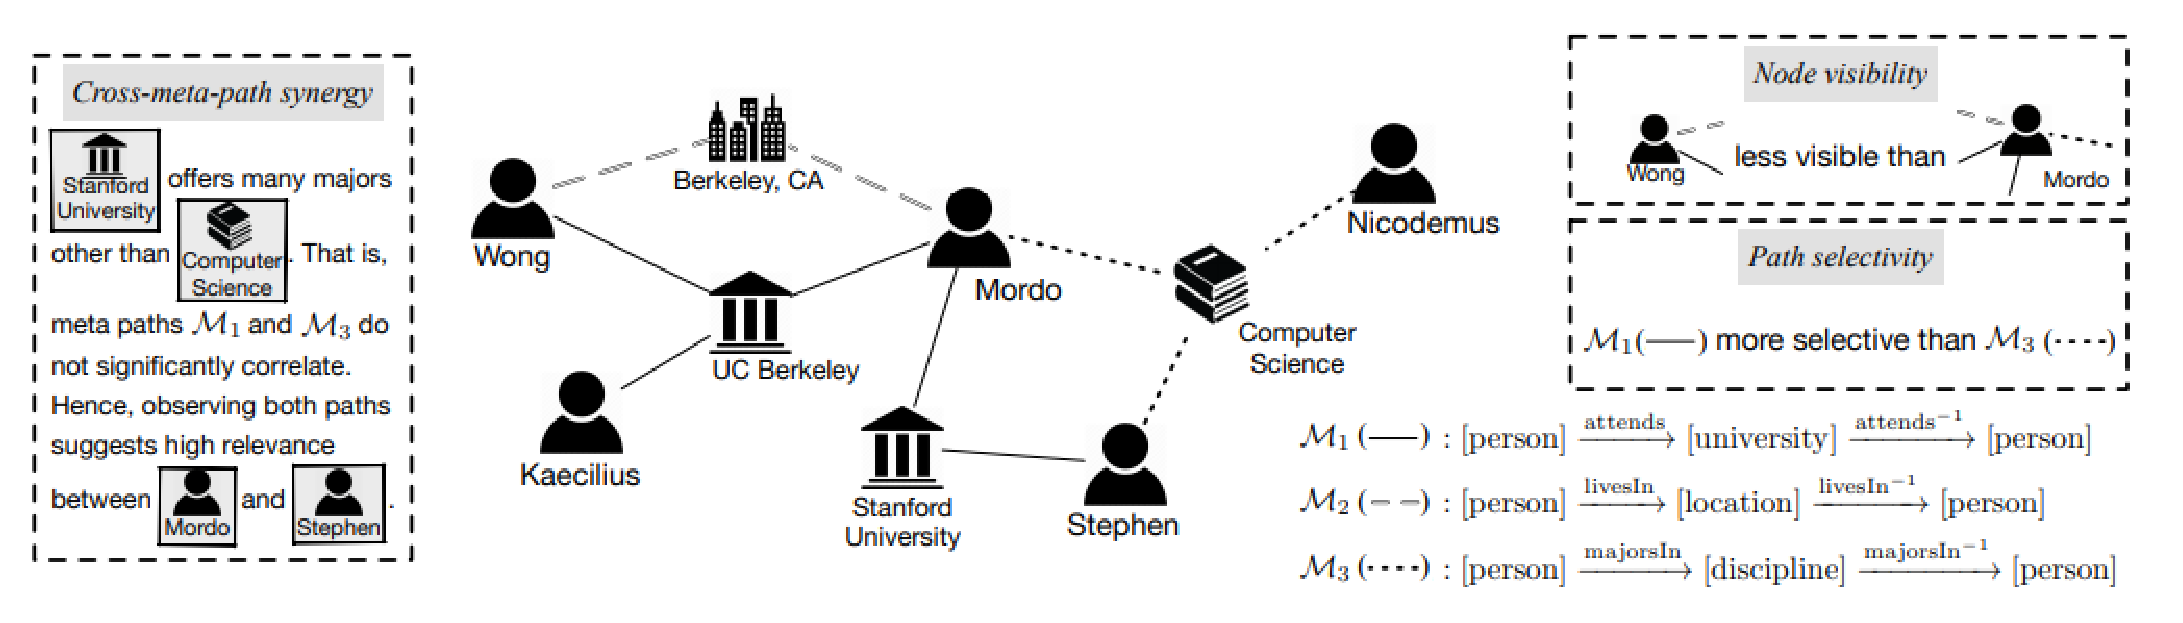
\includegraphics[height=4cm,width=1\textwidth]{fig1.eps}
		\caption{}
		\vspace{0pt}
	\end{figure} 
	
	A heterogeneous information network (HIN) is a network with varying types of objects that are interconnected. An example is shown un figure 1 where person, places, universities, and disciplines are in the same network. This networks are mathematically described by a graph $G = (V,E)$. The Path-based Relevance Probabilistic (PReP), in a nutshell, consists of two major parts: (i) inferring model parameters by finding the maximum a posteriori (MAP) estimate to fit the input HIN, and (ii) deriving relevance score between any node pair based on the learned model \cite{paper}. The two parts of the algorithm can be described as
	
	\begin{enumerate}
		\item \textbf{The Inference Algorithm:} Input the path counts $P$ and the parameters. Initialize the parameters $\rho, \Phi,$ and $\Theta$. While there hasnt been convergence, update the parameter $\eta$ by equation 10 in the paper. While $\eta$ has not converged, update $\rho_u$ by equation 11 in the paper for all $u$. Update $\Phi$ with equation 13 in paper and update $\theta$ with equation 12 in the paper.
		\item The relevance measure is given by
		$$ r(s) = \sum\limits_{t=1}^T \frac{P_{st}}{\rho_u\rho_\nu\eta_t\sum_{k-1}^K \phi_{sk}\theta_{kt}} + (1 - \beta)\sum\limits_{k=1}^K \log\phi_{sk} $$
		where the relevance is defined for all pairs of nodes.
	\end{enumerate}
	
	In terms of future work, the author alludes to a couple things in the paper
	
	\begin{enumerate}
		\item Sampling algorithm design to efficiently calculate marginal likelihood.
		\item Exploration of defining relevance from the proposed PReP model with marginal likelihood.
		\item Study on the cases with label information and meta-path selection.
	\end{enumerate}

	** I do not have a complete understanding of this paper so my strengths, weaknesses, and questions wont be too in depth ** \\

	Three strengths I found with the paper are
	\begin{enumerate}
		\item The results look better than current algorithms. 
		\item Real world applications of the algorithm lend itself to commercialization. 
		\item Algorithm can be parallelized, making it efficient.
	\end{enumerate} 
	\vspace{0.5cm}
	
	Three weaknesses I found with the paper are
	\begin{enumerate}
		\item The paper is not an easy read for those who lack a strong statistical background, making it hard for people to understand the research.
		\item I honestly can not determine other weaknesses since I had a hard time reading the paper.
	\end{enumerate}
	\vspace{0.5cm}
	
	Questions for the reader
	\begin{enumerate}
		\item I do not really have questions since the paper is unclear to me so I am hoping to understand the paper more in today's talk. 
	\end{enumerate}
	\vspace{0.5cm}
	
	\begin{thebibliography}{unsrt}
		\bibitem{paper}
		Yu Shi, Po-Wei Chan, Honglei Zhuang, Huan Gui, Jiawei Han \emph{PReP: Path-Based Relevance from a Probabilistic Perspective in Heterogeneous Information Networks}, KDD’17, August 13-17, 2017, Halifax, NS, Canada.
	\end{thebibliography}
	
\end{document}\documentclass[12pt]{article}